\begin{IEEEbiography}[{
\includegraphics[width=1in,height=1.25in,keepaspectratio]{authors_image/yanfei_liu.jpeg}}]{Yanfei Liu}
received the M.S. degree in computer application technology from Henan Polytechnic University, Jiaozuo, China, in 2008. She is currently an Associate Professor and the Program Director of the Artificial Intelligence Technology Application Program with the School of Information Engineering, Zhongshan Polytechnic, Zhongshan, China. She has presided over more than 20 research and education projects, including provincial key projects on citrus harvesting intelligent robots and a Zhongshan City key scientific research project entitled ``Research and Application of Dualarm Collaborative Intelligent Picking Robot for Pitaya Based on Deep Reinforcement Learning.'' Her research interests include agricultural robotics and dexterous manipulation, data-centric imitation learning, intelligent perception, and artificial intelligence technology education.
\end{IEEEbiography}

\begin{IEEEbiography}[{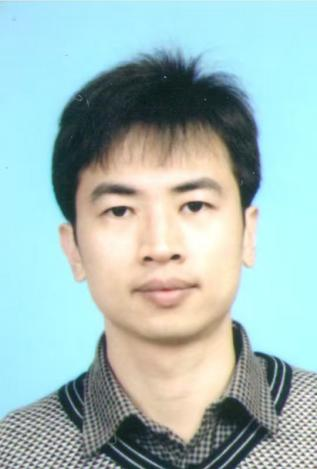
\includegraphics[width=1in,height=1.25in,keepaspectratio]{authors_image/liangzhong_lin.jpeg}}]{Liangzhong Lin}
received the Ph.D. degree in theoretical condensed matter physics from the Institute of Semiconductors, Chinese Academy of Sciences, Beijing, China, in 2014. He is currently a teacher of the Artificial Intelligence program at Zhongshan Polytechnic, Zhongshan, China. His research interests include the fundamental physics of semiconductors in mesoscopic systems, such as spin manipulation in two-dimensional electron gas (2DEG) and spin field effects in quasi-one-dimensional electron gas (Q1DEG), as well as semiconductor optoelectronics, intelligent LED control, AI technology applications, and data-centric intelligent systems.
\end{IEEEbiography}

\begin{IEEEbiography}[{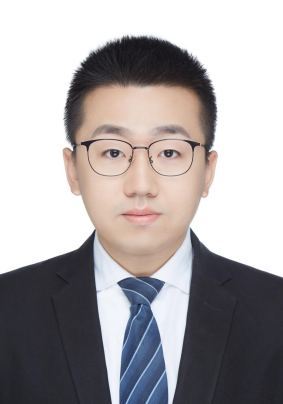
\includegraphics[width=1in,height=1.25in,keepaspectratio]{authors_image/zhiying_cao.png}}]{Zhiying Cao}
received the Ph.D. degree in signal and information processing from the University of Chinese Academy of Sciences. He used to be a Principal Algorithm Engineer and the Head of the Perception Model Development Section with the Automotive New Technology Research Institute, BYD Auto Industry Company Limited, Shenzhen, China. His research interests include data-centric autonomous driving perception, dataset quality governance, deep learning model compression, and computer vision.
\end{IEEEbiography}

\begin{IEEEbiography}[{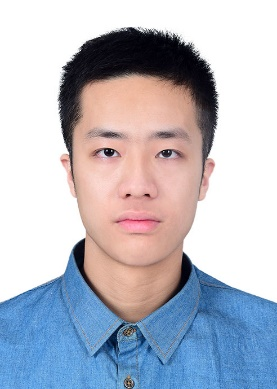
\includegraphics[width=1in,height=1.25in,keepaspectratio]{authors_image/chengliang_li.jpeg}}]{Chengliang Li}
is currently pursuing the B.S. degree in computer science and technology at Beijing Normal-Hong Kong Baptist University (BNBU), Zhuhai, China. He is an undergraduate student and expects to graduate in 2027. His research interests include robotics and embodied intelligence.
\end{IEEEbiography}

\begin{IEEEbiography}[{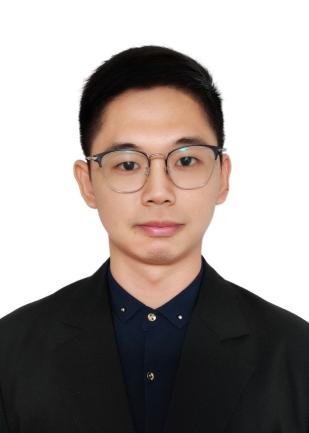
\includegraphics[width=1in,height=1.25in,keepaspectratio]{authors_image/weichang_li.jpeg}}]{Weichang Li}
received the B.S. degree and the M.Phil. degree in mechanical engineering from Guangdong University of Technology, Guangzhou, China, in 2019 and 2021, respectively. He is currently pursuing the Ph.D. degree in control engineering with the School of Automation Science and Engineering, South China University of Technology, Guangzhou, China. His research interests include the application of advanced control theory in real-world robotics.
\end{IEEEbiography}
